\section{Curvas}

\subsection{Curvas regulares, trazas, velocidades y tangencias}
\begin{defn}[Curva]
	$\gamma$ es una curva $\iff \appl{\gamma}{I=(a,b)\subseteq\R}{\R^3}$ es $C^{\infty}$
	\begin{itemize}
		\item Para casi todo lo que sigue basta con que $\gamma \in C^2$. Para contrastar, en alguna discusión posterior, admitiremos curvas que son solo $C^0 \ve C^1$.
		\item El intervalo $I = (a,b)$ puede ser no acotado en $\R$.
	\end{itemize}
\end{defn}
\begin{defn}[Traza]
	Sea $\gamma$ una curva, $\trz{\gamma}=\{\gamma(t):t\in I\}\subset \R^3$. También se dice que $\gamma$ es parametrización de $\trz{\gamma}$.
\end{defn}

\begin{obs}
	Dos curvas distintas pueden tener la misma traza y corresponden a parametrizaciones diferentes. De hecho, si $\appl{\gamma}{I}{\R^3}$ es una curva y $\appl{g}{J}{I}$ es una función sobreyectiva $C^{\infty}$
	\[\implies \appl{\mu}{J}{\R^3} : \mu(u)=\gamma\left(g(u)\right)\tex{ es una curva de misma traza que } \gamma\]
\end{obs}
\begin{defn}[Velocidad y rapidez]
	Sea $\appl{\gamma}{I}{\R^3}$ una curva, el vector velocidad (\allbold{velocidad}) de $\gamma$ en $t$ es $\gamma'(t)=\nabla\gamma(t)\in \R^3$. La norma $\norm{\gamma'(t)}$ se conoce como la \allbold{rapidez}.
\end{defn}
\begin{defn}[Curva regular]
	Sea $\appl{\gamma}{I}{\R^3}$, es regular $\iff \forall t \in I : \gamma'(t)\ne 0$
\end{defn}
\begin{ejem}
	El conjunto de puntos $V=\{(x, y)\in \R^2:-1<x<1\we y=|x|\}$ no es traza de ninguna curva regular.\\
	\indent Pongamos que $\gamma(t)=(x(t), y(t))$ es curva regular con traza $V$, y que $\gamma(0)=(0,0)$. Entonces $y(t)$ tiene un mínimo en $t = 0$ y $y'(0) = 0$. Si fuera $x'(0) > 0$, entonces $x(t) > 0$ para $t \in (0, \delta)$ y, por tanto, $x(t) =y(t)$ para $t \in \left[0, \delta\right)$ y, por tanto $x'(0) = y'(0) = 0$. Contradicción: la curva $\gamma$ no es regular. También conduce a contradicción el que $x'(0) = 0$.
\end{ejem}
\begin{defn}[Recta tangente a una curva regular]
	Sea $\appl{\gamma}{I}{\R^3}$ una curva regular y $t_0\in I$, $\appl{\eta}{\R}{\R^3}$ es la recta tangente a $\gamma$ en $\gamma(t) \iff \eta(u)=\gamma(t_0)+u\gamma'(t_0)$
\end{defn}

\subsection{Longitud de curvas y reparametrizaciones}
\subsubsection{Poligonales}
Sea $\appl{\gamma}{I}{\R^3}$ una curva (no necesariamente regular) y $\left[c, d\right] \subset I$. Definimos una poligonal de $\gamma$ entre $\gamma(c)$ y $\gamma(d)$ tomando una partición de $\left[c, d\right]$: $c=t_0<t_1<\cdots<t_{n-1}<t_n=d$.

La poligonal $\Pi$ asociada a esa partición es la lista de segmentos:
\[\Pi\defeq\left(\left[\gamma(t_0), \gamma(t_1)\right], \left[\gamma(t_1), \gamma(t_2)\right], \dots, \left[\gamma(t_{n-1}), \gamma(t_n)\right]\right)\]
La longitud de la poligonal $\Pi$ se denota $L(\Pi)$ se define entonces de forma natural como:
\[L(\Pi)=\sum_{j=1}^n \norm{\gamma(t_j)-\gamma(t_{j-1})}\]

\subsubsection{Definición de longitud de curva}
\begin{defn}[Longitud de una curva]
	Sea $\appl{\gamma}{I}{\R^3}$ una curva $C^0$, $\left[c,d\right] \subset  I$, se define la longitud como: \[\ds L(\gamma; c, d)=\sup \left\{L(\Pi) : \Pi\tex{ poligonal de } \gamma \tex{ entre }\gamma(c)\tex{ y }\gamma(d)\right\}\]
	En general, para una curva sólo continua este supremo puede ser $\infty$. Por ejemplo, para la curva copo de nieve de Von Koch.
\end{defn}

\subsubsection{Teorema de cálculo de longitud}
\begin{teo}
	Sea $\appl{\gamma}{I}{\R^3}$ una curva regular y $\ds \left[c,d\right] \subset  I \implies L(\gamma; c, d) = \int_c^d\norm{\gamma'(t)}\odif{t}$.
	\begin{dem}
		En la demostración denotamos
		\begin{itemize}
			\item $\ds L \defeq L(\gamma; c, d)$, que es supremo de las longitudes de las poligonales.
			\item $\ds J \defeq \int_c^d\norm{\gamma'(t)}\odif{t}$
		\end{itemize}
		Veamos que $\ds L\leq J \we J \leq L$:
		\begin{lem} \label{lem1}
			Sea $\appl{u}{I}{\R^3}$ una aplicación y sean $c, d \in I$, con $c<d$.
			\[\implies\norm{\int_c^du(t)\odif{t}} \leq \int_c^d\norm{u(t)}\odif{t}\]
		\end{lem}
		\begin{dem}
			Usamos que para cualquier $v$ se tiene $\ds\norm{v}=\sup\{|v\cdot w|:\norm{w}=1\}$. Pongamos $\ds v=\int_c^du(t)\odif{t}$ y sea $w$ con $\norm{w}=1$
			\[\implies v\cdot w=\int_c^d\left(u(t)\cdot w\right)\odif{t} \we \abs{v\cdot w}\leq\int_c^d\abs{u(t)\cdot w}  \odif{t} \leq  \int_c^d\norm{u(t)} \odif{t}\]
			Lo anterior es cierto para cualquier $w$ con $\norm{w}=1$.
		\end{dem}
		$\mathbf{\left[L\leq J\right]}$ Para una poligonal $\Pi$ con partición $t_0=c<t_1<\cdots<t_n=d$, se tiene que
		\[L(\Pi)=\sum_{j=1}^n\norm{\gamma(t_j)-\gamma(t_{j-1})} = \sum_{j=1}^n\norm{\int_{t_{j- 1}}^{t_j}\gamma'(t)\odif{t}}\]
		Por el Lema \ref{lem1}, se tiene $\ds L(\Pi) \leq \sum_{j=1}^n\int_{t_{j-1}}^{t_j}\norm{\gamma'(t)}\odif{t} =   \int_{t_0}^{t_n}\norm{\gamma'(t)}\odif{t} = J \implies L \leq J$.

		$\mathbf{\left[L\leq J\right]}$ Fijemos $\varepsilon > 0$. Por la continuidad uniforme de $\gamma'\in C^0$, $\exists \delta>0 : c\leq t\leq t'\leq d$ \\
		\centerline{\begin{itemize*}[itemjoin=\hspace{1cm}]
				\item son tales que $|t'-t|\leq \delta$
				\item entonces $\norm{\gamma(t')-\gamma(t)}\leq \varepsilon$
			\end{itemize*}}
		(El $\delta$ no depende de los puntos $t$ y $t'$, sólo de $\varepsilon$).

		Tomamos una partición $\ds t_0=c<t_1<\cdots <t_n=d$ para la que cumpla que $\ds t_j-t_{j-1}<\delta$ para $\ds j=1, \dots, n$. \\
		Sea $\Pi$ la poligonal dada por esa partición. Entonces:
		\[L(\Pi)=\sum_{j=0}^{n-1}\norm{\gamma(t_{j+1})-\gamma(t_j)}=\sum_{j=0}^{n-1}\norm{\int_{t_{j-1}}^{t_j}\gamma'(t)\odif{t}}\]
		Sea $\ds u_j\in \left[t_{j-1}, t_j\right]$ tal que $\ds\norm{\gamma'(u_j)}=\max_{t\in \left[t_{j-1}, t_j\right]}\norm{\gamma'(t)}$. \\
		Por un lado, $\ds J=\int_c^d\norm{\gamma'(t)}\odif{t} = \sum_{j=1}^n \int_{t_{j-1}}^{t_j}\norm{\gamma'(t)}\odif{t} \leq \sum_{j=1}^n\norm{\gamma'(u_j)}(t_j-t_{j-1}) \hspace{0.5cm} (\star)$ \\
		Por otro lado, \[\ds \gamma(t_{j+1})-\gamma(t_j) = \int_{t_j}^{t_{j+1}}\gamma'(t)\odif{t}=\left(\int_{t_j}^{t_{j+1}}(\gamma'(t)-\gamma'(u_j))\odif{t}\right)+\gamma'(u_j)(t_{j+1}-t_j)\]
		\begin{equation*}
			\begin{split}
				\implies \norm{\gamma(t_{j+1})-\gamma(t_j)} & \geq  \norm{\gamma'(u_j)}|t_{j+1}-t_j|-\norm{\int_{t_j}^{t_{j+1}}(\gamma'(t)-\gamma'(u_j))\odif{t}} \\ & \geq  \norm{\gamma'(u_j)}|t_{j+1}-t_j|-\varepsilon(t_{j+1}-t_j)
			\end{split}
		\end{equation*}
		usando el Lema \ref{lem1} y las condiciones de la partición.
		Por lo tanto, \begin{equation*}\begin{split}
				L(\Pi) & =\sum_{j=0}^{n-1}\norm{\gamma(t_{j+1}-\gamma(t_j))}
				\geq \sum_{j=0}^{n-1}\norm{\gamma'(u_j)}(t_{j+1}-t_j)-\varepsilon\sum_{j=0}^{n-1}(t_{j+1}-t_j) \geq J -\varepsilon(d-c)
			\end{split}\end{equation*}
		donde se ha usado $(\star)$. En suma $\ds \forall \varepsilon > 0 : J\leq L(\Pi) + \varepsilon(d-c)\geq L + \varepsilon(d-c) \implies J \leq L$.
	\end{dem}
\end{teo}
\begin{ejem}[Longitud gráfica de una función]
	$\ds \forall t \in \left[c, d\right] : \gamma(t)=(t, f(t))$ donde $\appl{f}{\left[c, d\right]}{\R}$ es una función deribable.
	\[\norm{\gamma'(t)}=\sqrt{1+(f'(t))^2} \implies \tex{Long gráfica }=\int_c^d \sqrt{1+(f'(t))^2} \odif{t}\]
\end{ejem}



\subsubsection{Reparametrizaciones}

Dada una curva $\appl{\gamma}{I}{\R^3}$, queremos recorrer su traza con otra curva.
\begin{defn}
	Sean $\appl{h}{J}{I}$ un difeomorfismo (biyección tal que tanto $h$ como $h^{-1}$ son $C^\infty$) y $\appl{\gamma}{I}{\R^3}$ una curva, $\appl{\eta}{J}{\R^3}$ es una reparametrización de $\gamma$
	\[ \iff \forall u \in J : \eta(u)=\gamma(h(u))\]
	\begin{itemize}[topsep=1pt, itemsep=1pt,parsep=3pt]
		\item $\eta$ es curva porque $\gamma$ lo es y $h$ es $C^\infty$.
		\item $\eta$ y $\gamma$ tienen la misma traza $(\trz{\eta}=\trz{\gamma})$.
		\item $\gamma$ es también reparametrización de $\eta$, pues $\gamma = \eta \circ h^{-1}$.
		\item $\eta$ regular $\iff \gamma$ regular, pues $\eta(u) = h'(u)\cdot\gamma'(h(u))$.
		\item En coordenadas, $\ds \frac{d}{du}\eta(u)=\big(\gamma_1'(h(u))\cdot h'(u),\, \gamma_2'(h(u))\cdot h'(u),\, \gamma_3'(h(u))\cdot h'(u)\big)$
	\end{itemize}
\end{defn}
\noindent \textbf{Orientación:}
\begin{itemize}[topsep=0pt, itemsep=1pt,parsep=3pt]
	\item Si $h$ es función creciente, entonces $\eta$ recorre la traza en el mismo sentido que $\gamma$.
	\item Si $h$ es decreciente, entonces $\eta$ recorre la traza en sentido contrario a como lo hace $\gamma$.
\end{itemize}
Supongamos que $h$ es creciente. Sean $\left[p, q\right]\subset J$. Llamamos $h(p)=c<d=h(q)$. La curva $\eta$ recorre de $p$ a $q$ la misma traza que $\gamma$ desde $c$ a $d$. La longitud de esa porción de traza se puede calcular con $\eta$ o con $\gamma$:
\[L(\gamma; c, d)=L(\eta; p, q) \iff \int_c^d\norm{\gamma'(t)}\odif{t}=\int_p^qh'(u)\norm{\gamma'(h(u))}\odif{u}\]

\subsubsection{Parametrización por longitud de arco}
\begin{defn}[Curva parametrizada por longitud de arco]
	Sea $\appl{\eta}{I}{\R^3}$ una curva regular, es parametrizada por longitud de arco
	\[\iff \forall s_1, s_2 \in I : s_1<s_2 : s_2-s_1=L(\eta; s_1, s_2)\]
	\[\iff \forall s_1, s_2 \in I : s_2-s_1=\int_{s_1}^{s_2}\norm{\eta'(d)}\odif{s} \iff \forall s \in I : \norm{\eta'(s)}=1\]
\end{defn}
\begin{teo}
	Toda curva regular se puede reparametrizar por longitud de arco.
	\begin{dem}
		Sea $\appl{\gamma}{I}{\R^3}$ una curva regular, fijamos $t_0\in I$ y defininimos: \[\forall t \in I : g(t)\defeq\int_{t_0}^t\norm{\gamma'(u)}\odif{u}\]
		\[\begin{cases}
				\tex{Para } t >t_0\tex{, se tiene que } g(t) \tex{ es la longitud de la curva } \gamma \tex{ entre } \gamma(t_0) \tex{ y } \gamma(t). \\
				\tex{Para } t <t_0\tex{, la función } g(t) \tex{ nos da el negativo de la longitud entre } \gamma(t_0) \tex{ y } \gamma(t).
			\end{cases}\]
		Queremos usar $s \defeq g(t)$ como etiqueta del punto $\gamma(t)$, en otras palabras, queremos despejar $t$ en términos de $s$, es decir, invertir $g$.
		\begin{itemize}
			\item Como $\gamma$ es regular, se tiene $g'(t)=\norm{\gamma'(t)}>0$. Así que $g$ es función creciente.
			\item Supongamos que $I=(a,b)$. Llamaremos $\ds c\defeq \lim_{t \rightarrow a}g(t)$ y $\ds d\defeq \lim_{t \rightarrow b}g(t)$
		\end{itemize}
		\[\implies \tex{La función $g$ es difeomorfismo entre $I=(a,b)$ y $J\defeq(c,d)$}\]
		\vspace{-1cm}
		\begin{lem}
			Sea $\appl{\alpha}{I}{\R^3}$ una función $C^\infty : \forall t\in I : \alpha(t)\ne 0 \implies \norm{\alpha(t)} \tex{es }C^\infty$
			\begin{dem}
				La función $\norm{\alpha(t)}^2=\alpha(t)\cdot\alpha(t)$ es $C^\infty$ y $\norm{\alpha(t)}$ es la raíz cuadrada de una función $C^\infty$ que no se anula, por tanto, es $C^\infty$.
			\end{dem}
		\end{lem}
		El lema nos da que $g'$ es $C^\infty$.
		Tomamos $\appl{h}{J}{I}$ dada por $h(s)\defeq g^{-1}(s)$, y consideramos la curva $\forall s \in J : \eta(s)\defeq\gamma(h(s))$. \\
		Se tiene que $\ds \eta'(s)=h'(s)\cdot\gamma'(h(s))=\frac{1}{g'(h(s))}\gamma'(h(s))=\frac{1}{\norm{\gamma'(h(s))}}\gamma'(h(s))$.
		\[\implies \forall s \in J : \norm{\eta'(s)}=1\implies \eta\tex{ está parametrizada por longitud de arco.}\]
	\end{dem}
\end{teo}
La relevancia del teorema de reparametrización por longitud de arco radica sobre todo en que nos permite suponer que hay tal reparametrización, no tanto en que sea un procedimiento para conseguirla.

\subsection{Curvatura y torsión}
La curvatura de una curva en un punto mide
\begin{itemize}[topsep=1pt, itemsep=1pt,parsep=3pt]
	\item cuán lejana está la curva de ser recta en ese punto.
	\item cuán rápidamente está cambiando de dirección en ese punto.
\end{itemize}
La torsión de una curva en un punto mide
\begin{itemize}[topsep=1pt, itemsep=1pt,parsep=3pt]
	\item cuán próxima está la curva a ser curva plana en ese punto.
	\item cuán rápidamente está cambiando su plano “osculador” en ese punto.
\end{itemize}
\begin{lem}
	\begin{enumerate}[topsep=0pt, itemsep=1pt,parsep=3pt]
		\item Sea $\appl{u}{I}{\R^3}$ una aplicación derivable tal que $\norm{u(t)}$ es constante en $I$.
		      \[\implies \forall t \in I : u'(t)\cdot u(t)=0 \iff \forall t \in I : u'(t) \perp u(t)\]
		\item Sean $\appl{u}{I}{\R^3}, \appl{v}{I}{\R^3}$ aplicaciones derivables tales que $u(t)\cdot v(t)=\tex{cte}$ en $I$.
		      \[\implies \forall t \in I : u'(t) \cdot v(t)=-u(t)\cdot v'(t)\]
	\end{enumerate}
	Uso típico: $\norm{u(t)}=1 \we u(t)\cdot v(t)=0$.
	\begin{dem}
		La primera parte del lema se deduce de la segunda, más general, tomando $v=u$.
		Como el producto escalar $u(t)\cdot v(t)$ es constante, derivando se tiene que
		\[\forall t \in I : u'(t)\cdot v(t) + u(t)\cdot v'(t) = 0 \implies \forall t \in I : u'(t)\cdot v(t) = - u(t)\cdot v'(t)\]
	\end{dem}
\end{lem}
\begin{defn}[Vector tangente]
	Sea $\appl{\gamma}{I}{\R^3}$ una curva parametrizada por longitud de arco ($\forall s \in I : \norm{\gamma'(s)}=1$), $\tngnt(s)$ es el vector tangente a $\gamma$ en $s\in I \iff \boxed{\tngnt(s)\defeq \gamma'(s)}$
\end{defn}
\begin{defn}[Curvatura] \label{defnCurvatura}
	Sea $\appl{\gamma}{I}{\R^3}$ una curva parametrizada por longitud de arco ($\forall s \in I : \norm{\gamma'(s)}=1$), $\kappa(s)$ es la curvatura de $\gamma$ en $s \in I \iff \boxed{\kappa(s) \defeq \norm{\tngnt'(s)}=\norm{\gamma''(s)}}$
\end{defn}

\begin{ejem}[Curvatura nula significa que la traza es (parte de) una recta]
	\mbox{ } \\
	Tenemos que $\kappa \equiv 0 \iff \tngnt' \equiv 0 \iff \tngnt = \gamma' \equiv \tex{cte} \iff \gamma(s) = \gamma(0) + s\tngnt(0)$ \[\iff \gamma \tex{ es parte de una recta.}\]
\end{ejem}

\begin{prop}
	Una curva en el plano de curvatura constante $M > 0$ está contenida en una circunferencia de radio $\sfrac{1}{M}$.
	\begin{dem}
		Sea $\appl{\gamma}{I}{\R^2}$ una curva parametrizada por longitud de arco en el plano con curvatura constante $M > 0$. Es decir, $\forall s \in I : \big(\norm{\gamma'(s)}=1 \we \norm{\gamma''(s)}=M\big)$.
		\begin{itemize}
			\item Como $\gamma'(s) \cdot \gamma'(s) \equiv 1$, se tiene $(\star)$ $\gamma''(s) \cdot \gamma'(s) \equiv 0$, es decir, $\gamma''(s) \perp \gamma'(s)$.
			\item Como $\gamma''(s) \cdot \gamma''(s) \equiv M^2$, se tiene que $\gamma''(s) \cdot \gamma'''(s) = 0$, es decir, $\gamma''(s) \perp \gamma'''(s)$.
		\end{itemize}
		Como $\gamma''(s) \neq 0$ (y dado que estamos en el plano), esto significa que $\gamma'''(s) \parallel \gamma'(s)$, \\
		es decir, $\gamma'''(s) = \lambda(s) \gamma'(s)$ para alguna función $\lambda(s)$ (de hecho, $\lambda(s) = \gamma'''(s) \cdot \gamma'(s)$).

		Derivamos en $(\star)$: $\gamma'''(s)\cdot \gamma'(s) + \gamma''(s)\cdot \gamma''(s) = 0 \implies \lambda(s) + M^2 = 0$.
		\[\implies \gamma'''(s) + M^2\gamma'(s)\equiv 0 \implies \frac{1}{M^2}\gamma'''(s) + \gamma'(s)\equiv 0 \implies \left(\gamma(s) + \frac{1}{M^2}\gamma''(s)\right)'\equiv 0\]
		De manera que existe un cierto $p\in \R^2$ tal que para todo $s\in I$
		\[\gamma(s) + \frac{1}{M^2}\gamma''(s) = p \implies \norm{\gamma(s) - p} = \frac{1}{M^2} \norm{\gamma''(s)} = \frac{1}{M}\]
		Concluimos que todos los puntos de la curva están a distancia $\sfrac{1}{M}$ de un cierto punto $p$, es decir, la curva está contenida en una circunferencia de radio $\sfrac{1}{M}$.
	\end{dem}
\end{prop}

\begin{defn}[Curva birregular]
	Sea $\appl{\gamma}{I}{\R^3}$ una curva regular, es birregular \[\ds\iff \forall s \in I : \gamma''(s) \ne 0 \iff\forall s \in I : \kappa(s)\ne 0\]
\end{defn}

\begin{prop}
	Una curva regular $\appl{\gamma}{I}{\R^3}$ (no necesariamente parametrizada por longitud de arco) es birregular $\iff \tex{su reparametrización por longitud de arco es birregular.}$
	\[\iff \forall i \in I : \gamma'(t)\tex{ y }\gamma''(t) \tex{ son linealmente independientes.}\]
	\begin{dem}
		Sea $\eta(s) = \gamma(h(s))$ una reparametrización de $\gamma$ por longitud de arco.
		\[\implies \eta'(s) = h'(s)\gamma'(h(s)) \,\, \we \,\, \eta''(s) = {h'(s)}^2\gamma''(h(s)) + h''(s)\gamma'(h(s))\]
		Si $\gamma$ es birregular, entonces $\eta$ también lo será y, por tanto, $\eta''(s) \ne 0$. \\
		Además, $\eta'(s)\cdot\eta''(s) = 0$, así que $\eta'(s)$ y $\eta''(s)$ son linealmente independientes. Mirando las expresiones de arriba, esto supone que $\gamma'(h(s))$ y $\gamma''(h(s))$ son linealmente independientes.

		Si $\gamma'(h(s))$ y $\gamma''(h(s))$ son linealmente independientes, entonces $\eta''(s)$ no puede ser el vector nulo, pues en la combinación lineal de arriba $h'(s) \ne 0$.
	\end{dem}
\end{prop}
\begin{defn}[Vector normal] \label{defnNormal}
	Sea $\appl{\gamma}{I}{\R^3}$ una curva birregular parametrizada por longitud de arco, $\nrml(s)$ es el vector normal a $\gamma$ en $s\in I$
	\[\iff\boxed{\nrml(s)\defeq\frac{\tngnt'(s)}{\norm{\tngnt'(s)}}= \frac{\gamma''(s)}{\norm{\gamma''(s)}}=\frac{\gamma''(s)}{\kappa(s)}}\]
	La aplicación $\appl{\operatorname{n}}{I}{\R^3}$ es $C^\infty$, pues $\kappa$ es $C^\infty$ y no se anula. \\
	Como $\norm{\tngnt}=1\implies \tngnt'(s)\perp \tngnt(s) \implies \boxed{\nrml(t) \perp \tngnt(s)}$ \\
	El vector $\nrml(s)$ es unitario y perpendicular a $\tngnt(s)$. Hay infinitos vectores en $\R^3$ (toda una circunferencia) con esa propiedad: $\nrml(s)$ es uno de ellos, pero canónico.
\end{defn}
\begin{defn}[Plano osculador]
	Sea $\appl{\gamma}{I}{\R^3}$ una curva parametrizada por longitud de arco, el subespacio afín $\pi$ es el plano osculador a la curva $\gamma$ en $s \in I$
	\[\iff \pi = \mathcal{L}\left\{\tngnt(s)=\gamma'(s), \nrml(s)=\frac{\gamma''(s)}{\kappa(s)}\right\} + \gamma(s) \]
	Para una curva en $\R^2$, el plano osculador es $\R^2$.
\end{defn}
Sea $\appl{\gamma}{I}{\R^3}$ una curva birregular parametrizada por longitud de arco y $0 \in I$. \\
La aproximación de primer orden a $\gamma$ en $\gamma(0)$ es la recta tangente a $\gamma$ en $\gamma(0)$:
\[\gamma(s)\approx\gamma(0) + s\gamma'(0)=\gamma(0)+s\tngnt()\]
La aproximación de segundo orden a $\gamma$ en $\gamma(0)$ se denomina \textbf{parábola osculatriz}:
\[\gamma(s)\approx\gamma(0) + s\tngnt(0) + \frac{1}{2}s^2\gamma''(0)=\gamma(0) + s\tngnt(0) + \frac{\kappa(0)}{2}s^2\nrml(0)\]
Entonces, ``hasta orden $2$'' la curva está contenida en su plano osculador.
\begin{defn}[Vector binormal]
	Sea $\appl{\gamma}{I}{\R^3}$ una curva birregular, $\bnrml(s)$ es el vector binormal a $\gamma$ en $s\in I \iff \boxed{\bnrml(s)\defeq\tngnt(s)\times\nrml(s)}$ \\
	Por las propiedades del producto vectorial $ \implies \bnrml(s) \perp \tngnt(s) \we \bnrml(s) \perp \nrml(s) \we \norm{\bnrml(s)}=1$.
	Entonces, el vector binormal es vector unitario normal al plano osculador a la curva en $s$.
\end{defn}
\begin{defn}[Triedro de Frenet]
	Sea $\appl{\gamma}{I}{\R^3}$ una curva birregular, el triedro de Frenet en $s\in I$ es la tripleta $\left(\tngnt(s), \nrml(s), \bnrml(s)\right)$
	\begin{itemize}
		\item $\forall s \in I : \left(\tngnt(s), \nrml(s), \bnrml(s)\right)$ es un triedro positivamente orientado.
		\item $\forall s \in I : \{\tngnt(s), \nrml(s), \bnrml(s)\}$ es una base ortonormal de $\R^3$.
	\end{itemize}
\end{defn}
La torsión de $\gamma$ en $s$ va a medir cómo varía el plano osculador a $\gamma$ en $s$ y, alternativamente, cuán ``plana'' es la curva $\gamma$ en $s$.

Como $\bnrml(s)$ es el vector normal al plano osculador a $\gamma$ en $s$, se trata de estudiar $\bnrml'(s)$. Sabiendo que $\bnrml(s)=\tngnt(s)\times\nrml(s)$, al derivar obtenemos:
\[\begin{aligned}
		\bnrml'(s) & =\tngnt'(s)\times\nrml(s)+\tngnt(s)\times\nrml'(s)                                    \\
		           & = \kappa(s)\nrml(s)\times\nrml(s)+\tngnt(s)\times\nrml'(s) = \tngnt(s)\times\nrml'(s)
	\end{aligned}\]
Se deduce que $\bnrml'(s) \perp \tngnt(s)$. Además, como $\bnrml(s)\cdot\bnrml(s)\equiv1 \implies \bnrml'(s)\perp\bnrml(s) \implies \bnrml'(s) \parallel \nrml(s)$.

\begin{defn}[Torsión] \label{defnTorsion}
	Sea $\appl{\gamma}{I}{\R^3}$ una curva birregular, $\tau(s)$ es la torsión de $\gamma$ en $\ds s\in I \iff \boxed{\bnrml'(s)=\tau(s)\nrml(s)} \implies \boxed{\tau(s)=\bnrml'(s)\cdot\nrml(s)} \we \norm{\bnrml(s)}=\abs{\tau(s)}$

	Para una curva birregular la curvatura es siempre positiva, pero la torsión en un punto dado puede ser positiva, negativa o 0. El signo de la torsión tiene significado geométrico.
\end{defn}
\begin{prop}[Torsión $\equiv 0$]
	Sea $\gamma$ una curva birregular,
	\[\gamma \tex{ está contenida en un plano} \iff \tau \equiv 0\]
	\begin{dem}
		$(\implies)$ Si la curva está contenida en un plano, entonces $\bnrml$ es constantemente uno de los dos vectores normales a dicho plano, por lo que $\bnrml' \equiv 0 \implies \tau \equiv 0$.

		$(\impliedby)$ Si $\tau \equiv 0$, entonces $\bnrml' \equiv 0 \implies \bnrml$ es constante. Por tanto, si fijamos $s_0\in I \implies \forall s \in I : \bnrml(s)=\bnrml(s_0)$. Queremos probar ahora que $\forall s \in I : (\gamma(s)- \gamma(s_0)) \perp \bnrml(s_0)$. \\
		Pero, derivando el producto escalar,
		\[\begin{aligned}
				((\gamma(s)-\gamma(s_0))\cdot\bnrml(s_0))' & = \gamma'(s)\cdot\bnrml(s_0)                                                      \\
				                                           & = \tngnt(s)\cdot\bnrml(s_0) =  \tngnt(s)\cdot\bnrml(s) = 0, \quad \forall s \in I
			\end{aligned}\]
		Por tanto, $(\gamma(s)-\gamma(s_0))\cdot\bnrml(s_0)$ es una constante cuando $s$ recorre $I$. Como en $s=s_0$ se anula, se tiene que $\forall s \in I : (\gamma(s)-\gamma(s_0))\perp\bnrml(s_0)$ y $\gamma$ está contenida en un plano.
	\end{dem}
\end{prop}
\begin{defn}[Planos]
	Sean $\appl{\gamma}{I}{\R^3}$ una curva parametrizada por longitud de arco y $(\tngnt, \nrml, \bnrml)$ su triedro de Frenet. Se definen
	\[\begin{aligned}
			\tex{Plano osculador, }    & \tex{determinado por} & \tngnt \we \nrml  \\
			\tex{Plano normal, }       & \tex{determinado por} & \nrml \we \bnrml  \\
			\tex{Plano rectificante, } & \tex{determinado por} & \tngnt \we \bnrml \\
		\end{aligned}\]
\end{defn}
\subsubsection{Fórmulas de Frenet-Serret}
Vamos a expresar las derivadas $\tngnt'(s), \nrml'(s), \bnrml'(s)$ respecto de la base $\{\tngnt(s), \nrml(s), \bnrml(s)\}$.

Ya tenemos $\tngnt'(s) = \kappa(s)\nrml(s) \we \bnrml'(s)=\tau(s)\nrml(s)$ de las definiciones \ref{defnCurvatura}, \ref{defnTorsion} y \ref{defnNormal}.
\[\bnrml(s)=\tngnt(s)\times\nrml(s) \implies \nrml(s) = \bnrml(s)\times\tngnt(s)\]
\[\begin{aligned}
		\implies \nrml'(s) & =\bnrml'(s)\times\tngnt(s) + \bnrml(s)\times\tngnt'(s) = \tau(s)\nrml(s)\times\tngnt(s) + \kappa(s)\bnrml(s)\times\nrml(s) \\
		                   & =-\tau(s)\bnrml(s)-\kappa(s)\tngnt(s)
	\end{aligned}\]
\[\implies \begin{pmatrix}
		\tngnt'(s) \\ \nrml'(s) \\ \bnrml'(s)
	\end{pmatrix} = \underbrace{\begin{pmatrix}
			0          & \kappa(s) & 0        \\
			-\kappa(s) & 0         & -\tau(s) \\
			0          & \tau(s)   & 0
		\end{pmatrix}}_{\eqdef FS}\begin{pmatrix}
		\tngnt(s) \\ \nrml(s) \\ \bnrml(s)
	\end{pmatrix}\]
Estas son las ecuaciones de Frenet-Serret donde la matriz escalar $FS$ es antisimétrica.

Si escribimos los vectores de arriba en coordenadas $(\tngnt=(t_1, t_2, t_3), \tngnt'=(t_1', t_2', t_3'), \tex{ etc.})$, la matriz anterior es de dimensiones $9\times9$: cada símbolo en la matriz $FS$ se ha de sustituir por una caja diagonal.

\subsubsection{Cambio de sentido y Triedro de Frenet}
Sea $\appl{\gamma}{I}{\R^3}$ una curva birregular parametrizada por longitud de arco. Supongamos por comodidad que $I = (-a, a) \implies 0\in I$ para $a>0$.

Consideramos la curva $\bar{\gamma}(s)\defeq\gamma(-s)$, que recorre la misma traza que $\gamma$, pero en sentido contrario. Queremos relacionar el tiedro de $\bar{\gamma}$ y su curvatura $\bar{\kappa}$ y torsión $\bar{\tau}$ con los de $\gamma$ en $0$, como $\bar{\gamma} (0)=\gamma(0)$:
\[\bar{\tngnt}(0)=-\tngnt(0) \we \bar{\nrml}(0)=\nrml(0) \we \bar{\kappa}(0)=\kappa(0) \we \bar{\bnrml}(0)=-\bnrml(0) \we \bar{\tau}(0)=-
	\tau(0)\]

\subsubsection{Movimientos rígidos y triedros}
Los movimientos rígidos de $\R^3$ se obtienen componiendo traslaciones con rotaciones. Si $M$ es movimiento rígido de $\R^3$, entonces $M$ viene dado por un vector $p$ y una matriz ortogonal $O$ $\left(O^T=O^{-1}\right)$ con determinante $1$:
\[\forall v \in \R^3 : M(v)=Ov+p\]
Como $|O|=1$, se tiene que $u, v \in \R^3 \implies Ou\times Ov=O(u\times v)$.
\begin{enumerate}
	\item \allbold{Traslaciones:} Sea $\gamma$ una curva birregular parametrizada por longitud de arco, definimos la curva $\bar{\gamma}(s)\defeq\gamma(s)+p$. \\
	      Como $\bar{\gamma}'(s)=\gamma'(s)$, se tiene que está parametrizada por longitud de arco \[\implies \forall s \in I : \bar{\tngnt}(s) = \tngnt(s) \we \bar{\kappa}(s)=\kappa(s) \we \bar{\nrml}(s)=\nrml(s) \we \bar{\tau}(s)=\tau(s) \we \bar{\bnrml}(s)=\bnrml(s)\]
	\item \allbold{Rotaciones:} Consideremos ahora la curva $\bar{\gamma}(s)=O\gamma(s)$. Se tiene $\bar{\gamma}'(s)=O\gamma'(s)$. \\Así que $\bar{\gamma}$ está parametrizada por longitud de arco y $\forall s \in I : \bar{\tngnt}(s)=O\tngnt(s)$.\\
	      Además, $\forall s \in I : \bar{\tngnt}'(s)=O\tngnt'(s) \implies \bar{\kappa}(s)=\kappa(s) \we \bar{\nrml}(s)=O\nrml(s)$
	      \[\bar{\bnrml}(s)=\bar{\tngnt}(s)\times\bar{\nrml}(s) = O\tngnt(s)\times O\nrml(s)=O\left(\tngnt(s)\times \nrml(s)\right)=O\bnrml(s) \implies \bar{\tau}(s)=\tau(s)\]
\end{enumerate}
Es decir, al trasladar o rotar la curva, sin deformarla, las longitudes se conservan: los triedros van en triedros y sus variaciones $(\kappa, \tau)$ se conservan.

\subsubsection{Otros triedros sobre curvas}

\begin{defn}[Tiedro positivo]
	Sea $\appl{\gamma}{I}{\R^3}$ una curva parametrizada por longitud de arco, $\left[P(s), Q(s), R(s)\right]$ es un triedro positivo sobre la curva $\gamma$.
	\[\iff \begin{cases}
			\appl{P, Q, R}{I}{\R^3} \quad C^\infty                  \\
			\forall s \in I : \norm{P(s)}=\norm{Q(s)}=\norm{R(s)}=1 \\
			\forall s \in I : P(s) \perp Q(s) \perp R(s) \we R(s) \perp P(s)
		\end{cases}\]
	Para cada $s \in I$ tenemos una base ortonormal $[P(s), Q(s), R(s)]$ de $\R^3$ positivamente orientada, i.e. $\forall s \in I : R(s)=P(s)\times Q(s)$.
\end{defn}

Vamos a expresar la variación de $[P(s), Q(s), R(s)]$ respecto de sí mismo.
\[\begin{pmatrix}
		P'(s) \\ Q'(s) \\ P'(s)
	\end{pmatrix} = \begin{pmatrix}
		\star & \star & \star \\
		\star & \star & \star \\
		\star & \star & \star \\
	\end{pmatrix}\begin{pmatrix}
		P(s) \\ Q(s) \\ R(s)
	\end{pmatrix}\]
Como $\norm{P(s)}\equiv1$, tenemos que $P'(s)\cdot P(s)=0$, análogamente para $Q$ y $R$. Así que la matriz tiene ceros en la diagonal.

Por otro lado, como $P(s)\cdot Q(s)=0 \implies P'(s)\cdot Q(s)=-Q'(s)\cdot P(s)$ y análogamente para $P(s)\cdot R(s)=0$ y $Q(s)\cdot R(s)=0$. Así que la matriz es antisimétrica.
\[\implies \begin{pmatrix}
		P'(s) \\ Q'(s) \\ P'(s)
	\end{pmatrix} = \begin{pmatrix}
		0     & A(s)  & B(s) \\
		-A(s) & 0     & C(s) \\
		-B(s) & -C(s) & 0    \\
	\end{pmatrix}\begin{pmatrix}
		P(s) \\ Q(s) \\ R(s)
	\end{pmatrix}\]
El el triedro de Frenet es un caso especialmente sencillo de tiedro positivo.

\subsection{Curvatura y torsión. Complementos}
\subsubsection{Curvas no parametrizadas por longitud de arco}
Sea $\appl{\gamma}{I}{\R}$ una curva con parámetro natural $t$ pero que no es longitud de arco. Queremos obtener la curvatura, torsión y el triedro de Frenet de $\gamma(t)$.

La parametrización $\eta$ por longitud de arco viene dada por $\forall t \in I : \gamma(t) = \eta(s(t))$ donde $s=s(t)$ es la longitud de arco de $\gamma$ desde $\gamma(t_0)$ hasta $\gamma(t)$.
\begin{center}
	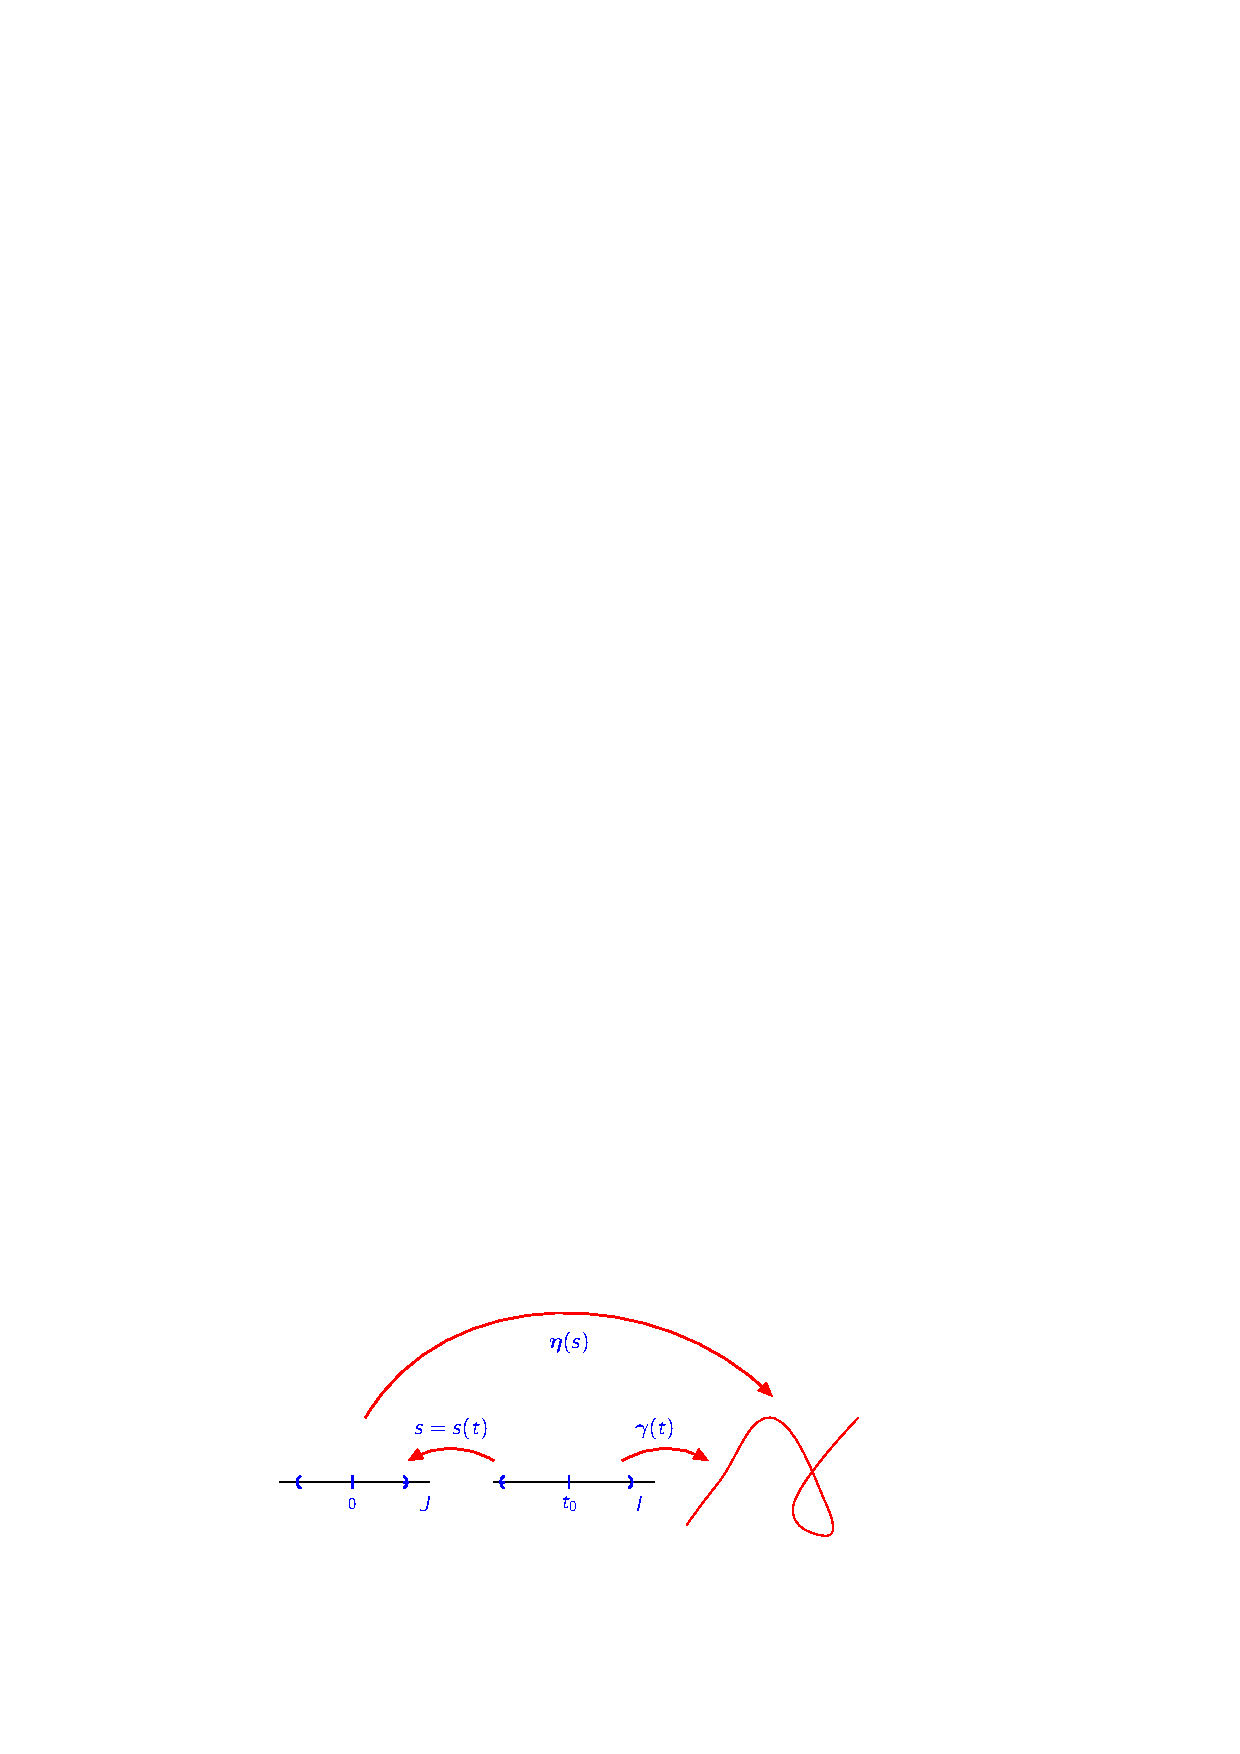
\includegraphics[width=8cm]{img/longarco}
\end{center}
Cuando $t$ recorre el intervalo $I$, el parámetro $s$ recorre un intervalo $J$. En notación general de (re)parametrización, la función $t \to s(t)$ se denota por $g(t)$.

Como $\tngnt, \nrml, \bnrml, \kappa, \tau$ se expresan y calculan a través de derivadas de $\eta$ y queremos hacerlo en términos de $\gamma$, aplicamos la regla de la cadena.

\[\forall t \in I : s(t) = \int_{t_0}^t \norm{\odv{\gamma}{t}(u)}\odif{u} \implies \forall t \in I : \odv{s}{t}(t)=\norm{\odv{\gamma}{t}(t)}\]
\[\odv{\gamma}{t}(t)=\odv{\eta}{s}(s(t))\cdot\odv{s}{t}(t)=\odv{s}{t}(t)\cdot\tngnt(s(t))\]
\[\implies \odv[2]{\gamma}{t} (t) = \left[\odv{s}{t}(t)\right]^2\cdot\odv{\tngnt}{s}(s) + \odv[2]{s}{t}(t)\cdot\tngnt(s) = \left[\odv{s}{t}(t)\right]^2 \kappa(s) \nrml(s) + \odv[2]{s}{t}(t)\cdot\tngnt(s)\]
\[\begin{aligned}
		\implies \odv[3]{\gamma}{t}(t) & = \kappa(s){\left(\odv{s}{t}(t)\right)}^3\odv{n}{s}(s)      & + \tex{ combinación lineal de $\tngnt$ y $\nrml$} \\
		                               & = - \kappa(s){\left(\odv{s}{t}(t)\right)}^3\tau(s)\bnrml(s) & + \tex{ combinación lineal de $\tngnt$ y $\nrml$}
	\end{aligned}\]

\textbf{Fórmula general para la curvatura}
\[\left(\odv{\gamma}{t}(t)\right)\times\left(\odv[2]{\gamma}{t}(t)\right)=\kappa(s)\left(\odv{s}{t}(t)\right)^3\bnrml(s) \implies \boxed{\kappa(s)=\frac{\norm{\gamma'\times \gamma''}}{\norm{\gamma'}^3}}\]
Para $\gamma$ parametrizada por longitud de arco $\norm{\gamma'}=1 \we \gamma'\perp\gamma'' \implies \kappa(s)=\norm{\gamma''(s)}$.

\textbf{Fórmula general para la torsión}
\[\begin{aligned}
		\left(\odv{\gamma}{t}(t)\times\odv[2]{\gamma}{t}(t)\right) \cdot \odv[3]{\gamma}{t}(t) & = \left(\kappa(s)\left(\odv{s}{t}(t)\right)^3\bnrml(s)\right)\cdot\left(-\kappa(s)\left(\odv{s}{t}(t)\right)^3\tau(s)\bnrml(s) + \dots \right) \\
		                                                                                       & = - \kappa^2\left(\odv{s}{t}(t)\right)^6\tau(s)=-\tau(s)\norm{\odv{\gamma}{t}(t)\times\odv[2]{\gamma}{t}(t)}^2
	\end{aligned}\]
\[\implies \boxed{\tau(s)=-\frac{(\gamma'\times\gamma'')\cdot\gamma'''}{\norm{\gamma'\times\gamma''}^2}}\]
En cuanto a $\tngnt$, $\nrml$, $\bnrml$:
\[\boxed{t=\frac{\gamma'}{\norm{\gamma'}}} \we \boxed{\bnrml=\frac{\gamma'\times\gamma''}{\norm{\gamma'\times\gamma''}}} \we \boxed{\nrml=\bnrml\times\tngnt=\frac{\left(\gamma'\times\gamma''\right)\times\gamma'}{\norm{\gamma'\times\gamma''}\norm{\gamma'}}}\]

\subsubsection{Curvatura de curvas planas}

Para curvas planas: podemos darle signo a la curvatura, y darle un significado geométrico.
\begin{defn}
	Sea $u \in \R^2$ un vector unitario $(\norm{u}=1)$, $u^\perp$ es el vector que se obtiene al girarlo $\sfrac{\pi}{2}$ en sentido positivo (antihorario) $\iff u=(\cos{\theta}, \sin{\theta}) \implies u^\perp=(-\sin{\theta}, \cos{\theta})$.
\end{defn}
Sea $\gamma$ una curva regular en $\R^2$ parametrizada por longitud de arco. \\
Denotamos con $\hat{\nrml}(s)\defeq{\tngnt(s)}^\perp$.
\[\implies \appl{\hat{\nrml}}{I}{\R^2} \quad C^\infty \we \forall s \in I : \left(\tngnt(s) \perp \hat{\nrml}(s)\right) \we \left(\nrml(s)=\pm \hat{\nrml}(s)\right)\]
Como $\tngnt'(s) \perp \tngnt(s)$, tenemos que $\tngnt'(s) \parallel \hat{\nrml}(s) \implies \tngnt'(s) = \hat{\kappa}(s) \cdot \hat{\nrml}(s)$. Donde $\hat{\kappa}(s)$ es la curvatura con signo de $\gamma$ en $s$.
La curvatura con signo solo requiere que la curva sea regular.
\[\implies \boxed{\hat{\kappa}(s)=\tngnt'(s)\cdot\hat{\nrml}(s)} \we \abs{\hat{\kappa}(s)}=\kappa(s)\]
El correspondiente vector binormal sería $\hat{\bnrml}=\tngnt\times\hat{\nrml}=\tngnt\times\tngnt^\perp=(0, 0, 1) \perp \R^2$.
\begin{center}
	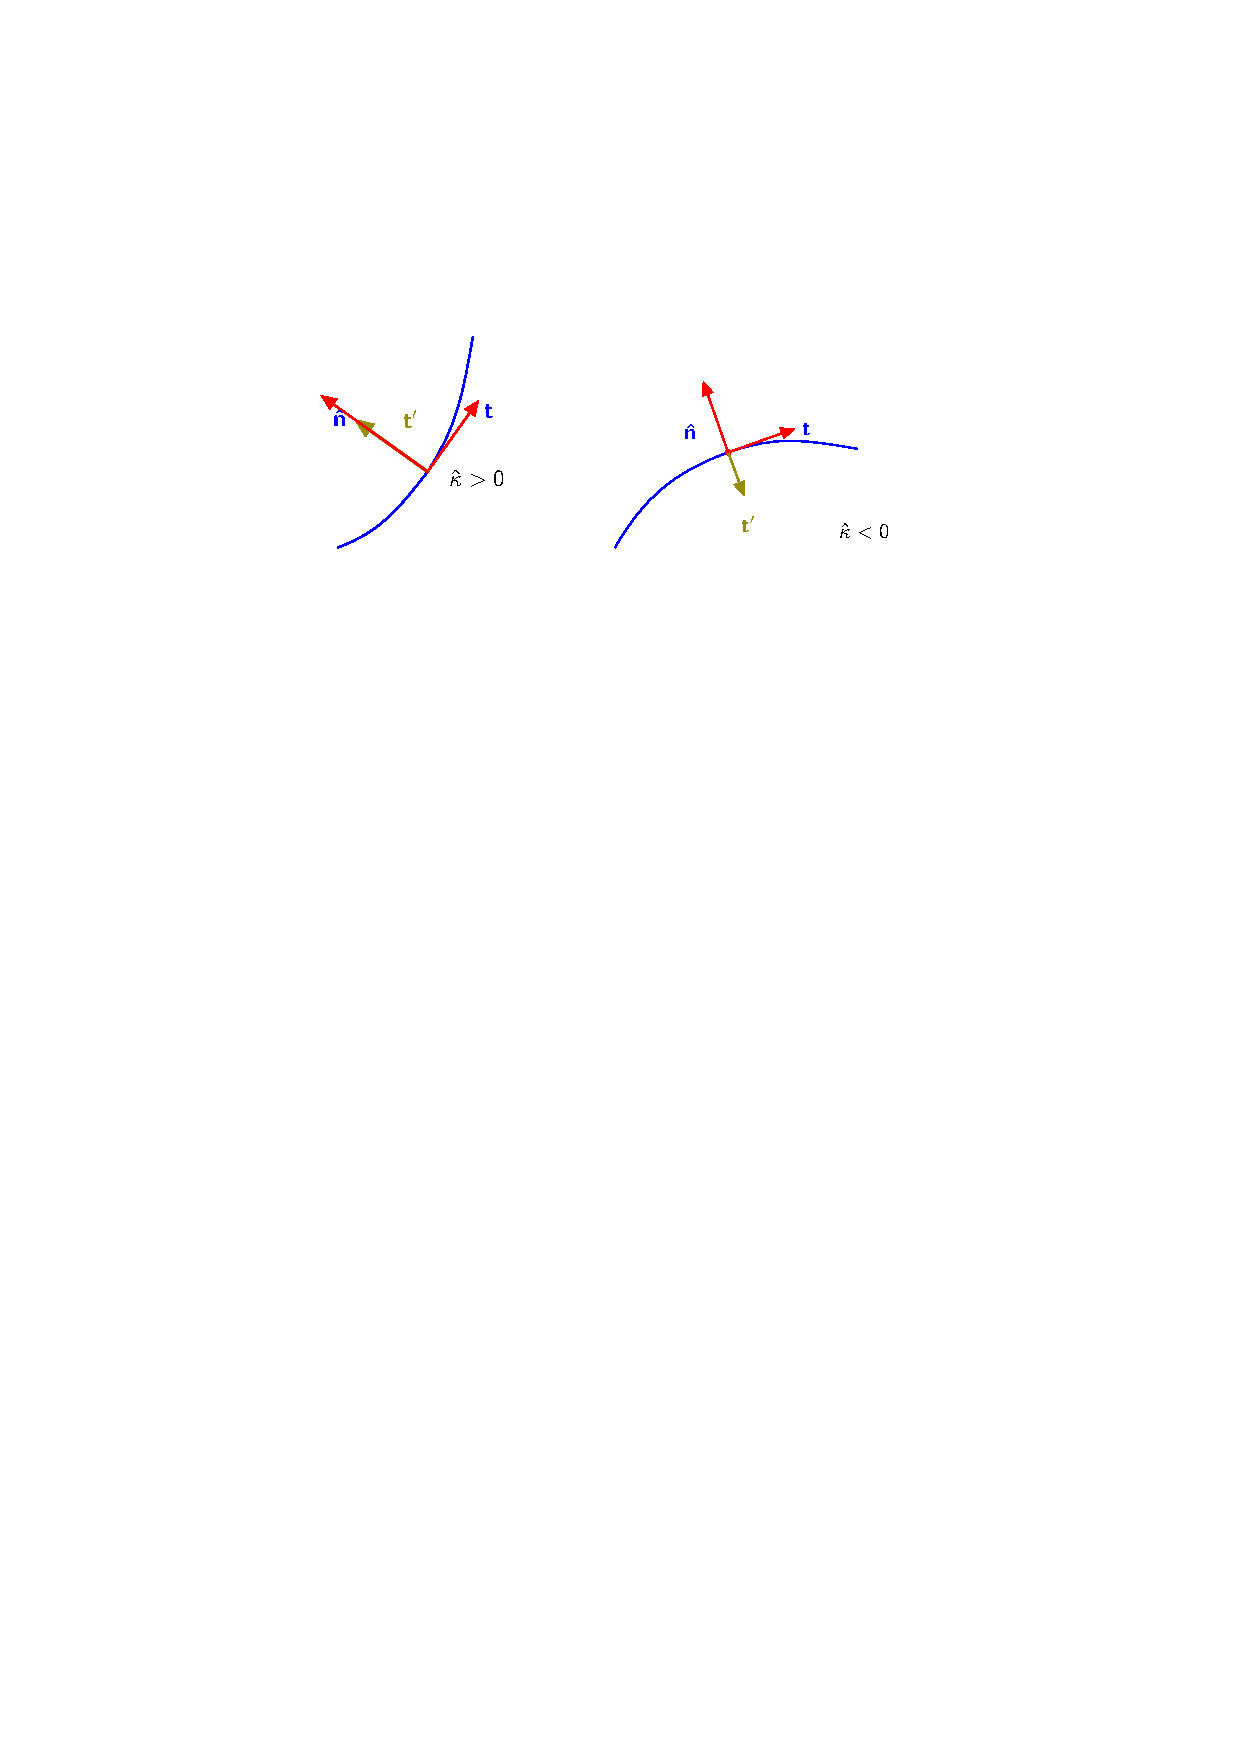
\includegraphics[width=10cm]{img/curvaturaR2}
\end{center}
Para una gráfica en el plano $t\mapsto (t, f(t))$ que se recorre de izquierda a derecha ($t$ creciente) la convexidad $(f'' > 0)$ corresponde con $\hat{\kappa} > 0$ y la concavidad corresponde con $\hat{\kappa} < 0$.

\textbf{Relación entre curvatura y ángulo con eje $OX$}

Vamos a describir la relación entre la curvatura $\hat{\kappa}$ y (la variación de) el ángulo que (el vector tangente de) la curva forma con el eje $OX$.

\begin{lem}
	Sea $\appl{u}{I}{\R^2}$ una aplicación $C^\infty : \forall t\in I : \norm{u(t)} = 1$.
	\[\implies \exists\, \appl{\theta}{I}{\R^2} \quad C^\infty : \forall t \in I : u(t)=(\cos{\theta(t)}, \sin{\theta(t)})\]
	La función $\theta$ es única salvo por adición de un múltiplo entero de $2\pi$. Por tanto, la derivada $\theta'$ está unívocamente determinada.
\end{lem}
Dada una curva $\gamma$ regular plana y parametrizada por longitud de arco, podemos escribir $\tngnt(s)=(\cos{\theta(t)}, \sin{\theta(t)})$ con $\theta$ función $C^\infty$. Así que, $\hat{\nrml}(s)=(-\sin{\theta(t)}, \cos{\theta(t)})$ donde $\theta(s)$ es el ángulo que forma $\tngnt(s)$ con el eje $OX$. El ángulo $\theta(s)$ determina la dirección de $\tngnt(s)$.
\[\implies \tngnt'(s)=\theta'(s)(-\sin{\theta(s)}, \cos{\theta(s)})=\theta'(s) \hat{\nrml}(s) \implies \forall s : \hat{\kappa}(s) = \theta'(s)\]

\textbf{Reconstrucción de curva plana a partir de $\hat{\kappa}$}

Sea $\appl{\gamma}{I}{\R^2}$ una curva plana parametrizada por longitud de arco y $M$ un movimiento rígido del plano que conserva orientación, es decir, una traslación compuesta con una rotación.

Consideremos la curva $\bar{\gamma}$ dada por $\forall s \in I : \bar{\gamma}(s)=M\gamma(s)$. Como $M$ es movimiento rígido, se tiene que $\bar{\gamma}(s)$ está parametrizada por longitud de arco y $\forall s \in I : \hat{\bar{\kappa}}(s)=\hat{\kappa}(s)$.

Ahora, como $\hat{\kappa}(s)=\theta'(s)$ y partimos de $\theta(0)=0 \implies \tngnt(0)=(1,0)$:
\[\implies \theta(s)=\int_{0}^{s}\theta'(u)\odif{u} = \int_0^s\hat{\kappa}(u) \odif{u}\]
Como $\gamma'(s)=\tngnt(s)=(\cos{\theta(s)}, \sin{\theta(s)})$, si establecemos $\gamma(0)=(0, 0)$
\[\implies\gamma(s)=\left(\int_0^s\cos{\theta(u)} \odif{u},\int_0^s\sin{\theta(u)} \odif{u}\right) \, \implies \, \boxed{\hat{\kappa} \Rrightarrow \theta' \Rrightarrow \theta \Rrightarrow \tngnt \Rrightarrow \gamma}\]
En general si conocemos la función $\ds \hat{\kappa}(s) \implies \theta(s) = \int \hat{\kappa}(s)\odif{s} + c_1$ para cierta constante $c_1$.
\[\implies \gamma(s)=\left(\int \cos{\theta(s)} \odif{s}, \int \sin{\theta(s)}\odif{s}\right) + (c_2, c_3) \tex{ para $c_2, c_3$ constantes.}\]
Los valores de $c_1, c_2, c_3$ quedan determinados, por ejemplo, por los valores de $\gamma$ y $\gamma'$ es un cierto $s_0\in I$.

\subsubsection{Forma canónica local}

Sea $\appl{\gamma}{I}{\R^3}$ una curva birregular parametrizada por longitud de arco.
Analizamos localmente, mediante aproximación de Taylor de tercer orden, la curva $\gamma$ en un entorno de $0 \in I$ centrado en $0$.
\[\gamma(s)=\gamma(0) + s\gamma'(0) + \frac{s^2}{2} \gamma''(0) + \frac{s^3}{6}\gamma'''(0) + E(s), \tex{ con }\lim_{s\to0}\frac{\norm{E(s)}}{s^3} = 0\]
\[\gamma(s)=\gamma(0) + \left(s-\frac{\kappa(0)^2s^3}{6}\right)\tngnt(0) + \left(\frac{\kappa(0)s^2}{2} + \frac{\kappa'(0)s^3}{6}\right)\nrml(0) + \left(-\frac{\kappa(0)\tau(0)s^3}{6}\right)\bnrml(0) + E(s)\]
Tras un movimiento rígido o con cambio de sistema de referencia, suponemos que
\[\gamma(0)=0 \we \tngnt(0)=i \we \nrml(0)=j \we \bnrml(0)=k\]
Si $\gamma(s)=(x(s), y(s), z(s))$ y si $E(s)=(e_x(s), e_y(s), e_z(s))$, entonces
\[\begin{cases}
		\ds x(s) & = s - \frac{\kappa(0)^2s^3}{6} + e_x(s)                     \\
		\ds y(s) & = \frac{\kappa(0)s^2}{2} + \frac{\kappa'(0)s^3}{6} + e_y(s) \\
		\ds z(s) & = -\frac{\kappa(0)\tau(0)s^3}{6} + e_z(s)
	\end{cases}\]
Esta es la forma canónica local de $\gamma$ cerca de $s=0$.

La torsión $\tau$ solo aparece en $z(s)$:
\begin{itemize}
	\item Si $\tau > 0$, para $s>0$ la curva $\gamma$ tiende a meterse debajo del plano osculador a $\gamma$ en $s=0$, donde ``debajo'' $=$ en dirección opuesta a $\bnrml$.
	\item Si $\tau < 0$, para $s>0$ la curva $\gamma$ tiende a pasar por encima del plano osculador a $\gamma$ en $s=0$, donde ``encima'' $=$ en la dirección de $\bnrml$.
\end{itemize}

\textbf{Forma canónica local. Curvas planas}

Sea $\appl{\gamma}{I}{\R^2}$ una curva parametrizada por longitud de arco con $0\in I$.
\[\implies \gamma(s)=\gamma(0)+s\tngnt(0)+\frac{s^2}{2}\hat{\kappa}(0)\hat{\nrml}(0) + F(s), \tex{ con } \lim_{s\to 0}\frac{\norm{F(s)}}{s^2} = 0\]
Con $\gamma(s)=(x(s), y(s)) \we \gamma(0)=(0,0) \we \tngnt(0)=(1, 0) \we \nrml(0)=(0,1)$ se tiene:
\[\begin{cases}
		x(s)=s-\frac{\kappa(0)s^3}{6}+o(s^3) \\
		y(s)=\frac{\kappa(0)}{2}s^2 + o(s^2)
	\end{cases}\]

\textbf{Circunferencia osculatriz}

\begin{itemize}
	\item Centro de curvatura $\ds \gamma(0) + \frac{1}{\kappa(0)}\nrml(0)$
	\item Radio de curvatura $\ds \frac{1}{\kappa(0)}$
\end{itemize}
La circunferencia osculatriz aproxima a la curva $\gamma$ cerca de $s=0$:
\[\norm{\gamma(s)-\left(\gamma(0) + \frac{1}{\kappa}\nrml(0)\right)}=\frac{1}{\kappa(0)} + o(s^2)\]

\textbf{Curvatura y comparación arco/cuerda en el plano}

Definimos $D(s)$ como la longitud del segmento (cuerda) que une $\gamma(s_0)$ con $\gamma(s)$: \[D(s)\defeq \norm{\gamma(s_0+s) - \gamma(s_0)}\]
\[\implies \begin{cases}
		\ds D(s) \leq \left[\tex{longitud de $\gamma$ entre $s_0$ y $s_0+s$}\right] = s \\
		\ds \lim_{s\to 0} \textstyle \frac{D(s)}{s} = \norm{\gamma'(s_0)} = 1
	\end{cases}\]
Poniendo $s_0=0$, y $\gamma(0)=(0,0) \we \tngnt(0)=(1, 0) \we \nrml(0)=(0, 1)$ se tiene
\[\begin{aligned} D(s)^2 = x(s)^2+y(s)^2 = s^2-2\frac{\kappa^2}{6}s^4 + \frac{\kappa^2}{4}s^4 + o(s^4) = s^2\left(1-\frac{1}{12}\kappa^2s^2+o(s^2)\right)\end{aligned}\]
Así que $\ds \frac{D(s)^2}{s^2} = 1-\frac{1}{12}\kappa^2s^2+o(s^2)$. Cuando más grande es $\kappa$, más pequeño es $\ds \frac{D(s)}{s}$

\subsection{Teorema fundamental de la teoría de curvas}

El \textbf{teorema fundamental de la teoría de curvas} afirma:
\begin{itemize}
	\item \textbf{Existencia:} Para cualesquiera posibles curvatura y torsión, hay una curva que las tiene como tales.
	\item \textbf{Unicidad:} La curvatura y la torsión de una curva la definen completamente salvo por la acción de un movimiento rígido.
\end{itemize}

\begin{teo}[Existencia]
	Sea $I$ un intervalo abierto y sean $\kappa (s)$ y $\tau (s)$ dos funciones $C^{\infty}$ en $I$ tales que $\forall s \in I : \kappa (s) >0$.

	Entonces, $\exists \appl{\gamma}{I}{\R^3}$ curva birregular parametrizada por longitud de arco tal que $\forall s \in I$ la curvatura y torsión de $\gamma$ en $s$ son $\kappa(s)$ y $\tau(s)$.
	\begin{dem}
		Apelaremos al siguiente resultado de ecuaciones diferenciales ordinarias: \vspace{-0.5cm}
		\begin{lem}
			Sea $I$ un intervalo abierto y, por comodidad, supongamos $0\in I$. Para cada $t\in I$, sea $\ds A(t)=\left(a_{ij}(t)\right)_{1\leq i, j\leq n}$ una matriz cuadrada de dimensiones $n\times n$ tal que las entradas $a_{ij}(t)$ son funciones $C^\infty$ en $I$. Sea $\bnrml_0 = (b_0, \dots, b_n)^T$ un vector $1\times n$.

			Entonces existe una única solución $\appl{X}{I}{\R^n}$ del problema de valores iniciales \[\ds \left\{X'(t)=A(t)X(t) \we X(0)=\bnrml_0\right\}\]
		\end{lem}
		Por comodidad, suponemos que $0\in I$. Sea $\left[P(s), Q(s), R(s)\right]$ solución del PVI de 9 ecuaciones diferenciales con 9 incógnitas:
		\[\begin{pmatrix}
				P'(s) \\ Q'(s) \\ R'(s)
			\end{pmatrix} = \begin{pmatrix}
				0          & \kappa(s) & 0        \\
				-\kappa(s) & 0         & -\tau(s) \\
				0          & \tau(s)   & 0
			\end{pmatrix}\begin{pmatrix}
				P(s) \\ Q(s) \\ R(s)
			\end{pmatrix} \,\, \we \,\, \begin{pmatrix}
				P(0) \\ Q(0) \\ R(0)
			\end{pmatrix} = \begin{pmatrix}
				(1,0,0) \\ (0,1,0) \\ (0,0,1)
			\end{pmatrix}\]
		Consideramos los seis productos escalares:
		\[\begin{pmatrix} (P \cdot Q)' \\ (P \cdot R)' \\ (Q \cdot R)' \\ (P \cdot P)' \\ (Q \cdot Q)' \\ (R \cdot R)' \end{pmatrix} = \begin{pmatrix} 0        & - \tau   & 0      & - \kappa & \kappa & 0      \\
                \tau     & 0        & \kappa & 0        & 0      & 0      \\
                0        & - \kappa & 0      & 0        & \tau   & - \tau \\
                2\kappa  & 0        & 0      & 0        & 0      & 0      \\
                -2\kappa & 0        & -2\tau & 0        & 0      & 0      \\
                0        & 0        & 2\tau  & 0        & 0      & 0
			\end{pmatrix}\begin{pmatrix} (P \cdot Q) \\ (P \cdot R) \\ (Q \cdot R) \\ (P \cdot P) \\ (Q \cdot Q) \\ (R \cdot R) \end{pmatrix} \we \begin{pmatrix}
				(P \cdot Q)(0) \\ (P \cdot R)(0) \\ (Q \cdot R)(0) \\ (P \cdot P)(0) \\ (Q \cdot Q)(0) \\ (R \cdot R)(0)
			\end{pmatrix} = \begin{pmatrix}
				0 \\ 0 \\ 0 \\ 1 \\ 1 \\ 1
			\end{pmatrix}\]
		Por unicidad de este sistema de ecuaciones diferencias, se tiene que
		\[(P\cdot Q) = 0 \we (P\cdot R) = 0 \we (Q\cdot R) = 0 \we (P\cdot P) = 1 \we (Q\cdot Q) = 1 \we (R\cdot R) = 1\]
		Por tanto, $\left[P(s), Q(s), R(s)\right]$ es un triedro ortonormal positivo.

		Sea ahora $\gamma$ dada por $\gamma'(s) = P(s)$ y $\gamma(0)=0$. \\
		Como $\norm{P} \equiv 1$, se tiene que $\gamma$ está parametrizada por longitud de arco. \\
		Además, como $\gamma''\equiv P \equiv \kappa Q$ y $\norm{Q}\equiv 1$, se tiene que $\kappa$ es la curvatura de $\gamma$ y $\nrml = Q$. \\
		Como $R\equiv P \times Q$, por ser triedro positivo, se tiene que $\bnrml = R$. \\
		Por último, como $\bnrml' = R' = \tau \nrml$, se tiene que $\tau$ es la torsión de $\gamma$.
	\end{dem}
\end{teo}

\begin{teo}[Unicidad salvo movimiento rígido]
	Sean $\gamma$ y $\Bar{\gamma}$ dos curvas definidas en $I$ y parametrizadas por longitud de arco.
	\[\forall s \in I : \kappa(s)=\Bar{\kappa}(s) \we \tau(s) = \Bar{\tau}(s) \iff \exists M \tex{ movimiento rígido} : \forall s \in I : \bar\gamma (s) = M \gamma (s)\]
	\begin{dem}
		$(\impliedby)$ Ya se ha visto.

		$(\implies)$ Suponemos sin pérdida de generalidad y por comodidad que $0\in I$. \\
		Suponemos, además, que $\gamma(0)=\bar{\gamma}(0)$, $\tngnt(0)=\bar{\tngnt}(0)$, $\nrml(0)=\bar{\nrml}(0)$ y $\bnrml(0)=\bar{\bnrml}(0)$.
		\begin{itemize}
			\item Tras esta normalización, queremos probar que $\gamma(s)=\bar{\gamma}(s)$ para todo $s\in I$.
			\item Comprobaremos que $\forall s \in I : \tngnt(s)=\bar{\tngnt}'(s)$. Con esto bastará porque integrando y usando que $\gamma(0)=\bar{\gamma}(0)$ se tiene que $\gamma(s)=\bar{\gamma}(s)$.
			\item De hecho, probaremos simultáneamente que $\forall s \in I : \nrml(s)=\bar{\nrml}(s) \we \bnrml(s)=\bar{\bnrml}(s)$.
		\end{itemize}
		Consideramos la función real $h$ definida en el intervalo $I$.
		\[h(s)\defeq \frac{1}{2} \left(\norm{\tngnt(s)-\bar{\tngnt}(s)}^2 + \norm{\nrml(s)-\bar{\nrml}(s)}^2 + \norm{\bnrml(s)-\bar{\bnrml}(s)}^2\right)\]
		Queremos ver que $h(s)\equiv 0$. Como $h(0)=0$, basta probar que $h'(s)\equiv 0$.

		Derivando y usando las fórmulas de Frenet-Serret y que $\kappa(s)=\bar{\kappa}(s)$ y $\tau(s)=\bar{\tau}(s)$, se tiene que (obviando el parámetro $s$):
		\[\begin{aligned}
				h' & = (\tngnt' - \bar{\tngnt}')\cdot(\tngnt - \bar{\tngnt}) + (\nrml' - \bar{\nrml}')\cdot(\nrml - \bar{\nrml}) + (\bnrml' - \bar{\bnrml}')\cdot(\bnrml - \bar{\bnrml})                                                                    \\
				   & = \kappa(\nrml - \bar{\nrml})\cdot(\tngnt - \bar{\tngnt}) - \kappa (\tngnt - \bar{\tngnt})\cdot(\nrml - \bar{\nrml}) - \tau (\bnrml - \bar{\bnrml})\cdot(\nrml - \bar{\nrml}) + \tau (\nrml - \bar{\nrml})\cdot(\bnrml - \bar{\bnrml}) \\
				   & = 0 \implies h' \equiv 0
			\end{aligned}\]
	\end{dem}
\end{teo}

\subsection{Desigualdad isoperimétrica. Geometría global de curvas planas}

\allbold{Problema isoperimétrico:} de entre todas las figuras planas con idéntico perímetro, ¿cuál es la que encierra mayor área?

La desigualdad afirma que dada la longitud $L$ de una curva simple cerrada $\gamma$, hay una cota superior $\ds \varphi(L) = \frac{\pi}{4}L^2$ para el área $A$ encerrada por $\gamma$.

Pero no queremos una cota, queremos la mejor cota posible.
\[\Phi (L) \defeq \sup\{A : A \tex{ es el área encerrada por una curva simple cerrada de longitud }L\}\]
\begin{itemize}
	\item Cota superior para $\Phi$: ya sabemos que $\Phi \leq \varphi$.
	\item Cota inferior para $\Phi$: pongamos que $\gamma$ es una circunferencia de radio $R$. En este caso, $L=2\pi R$ y $A=\pi R^2$. Así que $\Phi(L) \geq \frac{1}{4\pi}L^2$.
\end{itemize}
\[\implies \frac{1}{4\pi}L^2 \leq \Phi(L) \leq \frac{\pi}{4}L^2\]
Vamos a comprobar que la función $\Phi$ tiene que ser $\Phi(L) = C L^2$ para alguna constante $C$.

Una homotecia de razón $r>0$ lleva la curva $\gamma$ en la curva $r\gamma$ y el área encerrada y la longitud de la curva se transforman como $r^2$ y $r$ respectivamente. Así que:
\[r^2A \leq \Phi(rL) \implies r^2\Phi(L) \leq \Phi(rL) \implies \frac{1}{r^2}\Phi(rL) \leq \Phi(L) \implies r^2\Phi(L) \geq \Phi(rL)\]
Con $r=\sfrac{1}{L}$ se tiene que $\ds \Phi(1) \leq \frac{1}{L} \Phi(L) \leq \Phi(1) \implies \Phi(L) = \Phi(1) L^2$.

\subsubsection{Conceptos varios}
\begin{enumerate}
	\item Una \textbf{curva simple cerrada plana} $\gamma$ de periodo $a>0$ es una curva \\$\appl{\gamma}{\R}{\R^{3}}$ tal que $\ds \gamma (t_{1})=\gamma(t_{2}) \iff \frac{t_{1}-t_{2}}{a}\in \Z$.
	      \begin{itemize}
		      \item La traza de $\gamma$ es $\gamma (\R)=\gamma ([0,a))$.
		      \item La aplicación $\gamma$ es inyectiva en el intervalo $[u,u+a)$ sea cual sea $u$.
		      \item La longitud $L$ de $\gamma$ es $\ds \int_{0}^{a}\|\gamma '(t)\|dt$.
		      \item Si $\gamma$ es regular y está parametrizada por longitud de arco, entonces $a = L$.
	      \end{itemize}
	\item \textbf{Región encerrada: El teorema de la curva de Jordan:}

	      La traza de una curva simple cerrada plana $\gamma$ separa el plano en exactamente dos componentes conexas. Una de ellas es acotada y la otra no.

	\item \textbf{Área encerrada. Fórmula de Green:}

	      La fórmula de Green nos dice que si $\gamma (t)=(x(t),y(t))$ recorrida en sentido positivo encierra la región $\mathcal{I}$, entonces \[\iint_{\mathcal{I}} (Q_{x}-P_{y})\odif{x}\odif{y}=\int_{\gamma}(P\odif{x}+Q\odif{y})\]
	      Recordamos aquí que si $\gamma (t)=(x(t),y(t)), t\in (a,b)$ entonces \[\int_{\gamma} (P\odif{x}+Q\odif{y})=\int_{a}^{b} (P(x(t),y(t)) \cdot x'(t) + Q(x(t),y(t))\cdot y'(t))\odif{t}\]

	      Si tomamos $\ds Q(x,y)=x \we P\equiv 0 \implies \tex{Área}(\mathcal{I}) = \int_{\gamma} x \odif{y} = \int_{a}^{b} x(t)y'(t)\odif{t}$.

	      Si tomamos $\ds p(x,y)-y \we Q\equiv 0 \implies \tex{Área}(\mathcal{I}) = -\int_{\gamma} y \odif{x} = - \int_{a}^{b} y(t)x'(t)\odif{t}$.
	      \[\implies \tex{Área}(I)=\frac{1}{2}\int_{\gamma}(xdy-ydx)=\frac{1}{2}\int (x(t)y'(t)-y(t)x'(t)) dt\]
\end{enumerate}